\documentclass{msuphddissertation}
\usepackage{amsmath}
\usepackage{amsfonts}
\usepackage{graphicx}
%\usepackage{hyperref}
\usepackage{enumitem}
\usepackage{minibox}
\usepackage{color}
\usepackage{siunitx}\sisetup{per-mode=symbol}
%\usepackage{tabularx}
\usepackage{listings}
%	QUOTE ENVIRONMENT    
\usepackage[T1]{fontenc}
\usepackage{xparse}
\usepackage{enumitem}
\setlist[description]{
  font={\bfseries},
  labelsep=0pt,
  labelwidth=\transcriptlen,
  leftmargin=\transcriptlen,
}

\newlength{\transcriptlen}

\NewDocumentCommand {\setspeaker} { mo } {%
  \IfNoValueTF{#2}
  {\expandafter\newcommand\csname#1\endcsname{\item[#1:]}}%
  {\expandafter\newcommand\csname#1\endcsname{\item[#2:]}}%
  \IfNoValueTF{#2}
  {\settowidth{\transcriptlen}{#1}}%
  {\settowidth{\transcriptlen}{#2}}%
}

\setspeaker{SA}
\setspeaker{SB}
\setspeaker{SC}
\setspeaker{SD}
\setspeaker{TA}

\addtolength{\transcriptlen}{1em}

%
%	FRONT
%

\author{Michael J. Obsniuk}
\title{Identifying Computational Practices in Introductory Physics}
\unit{Physics --- Doctor of Philosophy}

\begin{document}

\maketitlepage

\begin{abstract}
\end{abstract}

\TOC
\LOT
\LOF

\newpage
\pagenumbering{arabic}
\begin{doublespace}

%
%	INTRODUCTION (VERY HIGH LEVEL)
%

\chapter{Introduction}\label{CH1:Introduction}

Since the advent of relatively inexpensive and powerful computers, researchers have been interested in their use as both professional and pedagogical tools.  Their ability to quickly and precisely perform numerical calculation makes them well suited for modeling and solving modern problems in the STEM fields.  Similarly, their ability to easily generate meaningful visualizations makes them well suited for the communication of scientific information.  For these reasons, computation is indispensible in modern scientific pursuits.

Computation, or the use of computers to analyze complicated problems, continues to grow in many fields, from mathematics to biology.  Given its utility in these professional domains, the task of effectively training students in computation has risen to the forefront of education research.  This task has been shown to involve many challenges, as there are many and varied skills and pieces of knowledge that students must develop a mastery of in order to effectively utilize computation.  Still, the desire to integrate computation into the STEM curriculum is stronger than ever.

While using computation to solve complex physics and engineering problems, practitioners often engage in various computational practices.  Computational practices can be defined as a synthesis of computational knowledge and computational skill -- highlightning the importance of being able to put theoretical ideas to practical work.  Although knowledge and skill alone are important, being able to combine the two into an effective \textit{practice} is even moreso.  Although attempts have been made to define computational practices broadly, they are still lacking clear and precise definition within many particular domains (e.g., computational physics). Accordingly, this thesis focuses on identifying the common computational physics practices that students engage in while solving realistic physics and engineering problems.

% For each reason, add a reference and example.

There are a number of reasons for focusing on computational physics and its associated computational practices.  Perhaps most important is that there is a high demand for computational skills in the workplace for physics graduates \cite{AAPT2016}.  Being able to effectively prepare students requires in-depth research to develop best practices.  Modern physics curricula should reflect the modern practices of professional physicists, and computation is often seen as just as important as theory and experiment.  For this reason, $\SI{51}{\percent}$ of faculty from physics departments call for more computation in the curriculum \cite{Chonacky2008}.

Additionally, it is believed that students of computational physics gain a deeper understanding of the physical concepts \cite{Chabay2008,Kohlmyer2005}.  Visual packages such as VPython or Glowscript \cite{Sherer2000} allow novice programmers to create stunning three-dimensional visualizations that allow them to more easily interact with the fundamental concepts.

Further, computation allows for the analysis of realistic problems that have no closed-form solution.  Its ability to numerically integrate supports a more exploratory approach to analyzing physical systems and learning physics.  That is, the repeated application of Newton's second law allows for a more general analysis.  This more exploratory approach is thought to encourage students to construct more realistic and accurate computational models through computational thinking \cite{AAPT2016}.

Finally, computational thinking is a term that has become increasingly popular since its introduction in the early 1980s.  This term, although frequently used today, is difficult to concisely explain given its many and varied definitions.  Even within the fields of education and computer science, many different viewpoints exist on the topic, and the corresponding definitions are just as varied \cite{Grover2013}.  However, many of these definitions share one fundamental characteristic: solving complex problems through abstraction and analytic thinking with the aid of computer algorithms, which is precisely the type of thinking that this thesis explores.

Computational thinking is so highly valued by the modern enterprise of science education that the Next Generation Science Standards (NGSS) laid out a framework for identifying computational thinking in K-12 settings.  As early as the fifth grade students are expected to be able to think computationally.  They describe computational thinking, at this level, in terms of analyzing data and comparing approaches.  By the time students reach middle school, computational thinking advances to analyzing large data sets and generating explanations.  Finally, in high school, computational thinking expands to constructing computational models and using them to answer questions \cite{NGSS2012}.  Clearly, computational thinking is a complicated concept which requires substantial explanation.

Experts in the field still have a ways to go when it comes to clearly defining computational thinking within science education, and, within physics education, specifically.  However defined, though, this type of abstract and algorithmic thinking is pervasive -- it extends beyond computer science into fields from geology to astronomy, and even beyond STEM \cite{Bundy2007}.  It is becoming increasingly clear that ``computational thinking is a fundamental skill for everyone, not just computer scientists \cite{Wing2006}.''

Given the recent interest in scientific practices, and computational thinking more specifically, a taxonomy of the computational practices indicative of computational thinking has been proposed \cite{Weintrop2015}.  This taxonomy, comprised of twenty-two individual yet inter-related practices, fitting into four different categories, is meant to help guide instructors and researchers as they attempt to teach and better understand computational thinking in science classrooms.  Each practice, according to the taxonomy, is defined broadly and from an expert level so as to be applicable to a wide range of science classrooms.

However, the broad and expert-generated definitions that make the taxonomy widely applicable also leave it relatively vague and difficult to apply to any particular situation.  Reducing the vagueness and difficulty of applying this taxonomy to a specific domain of inquiry (i.e., introductory physics) is a challenging but important task.  Having a taxonomy that is both precise and easy to apply will provide a solid foundation for instructors to generate/validate computational problems and for researchers to analyze the learning process.  \textbf{Accordingly, it is important that we identify, through direct observation, the set of computational practices that are common to computational introductory physics.}  This involves not only identifying the practices, but also the underlying knowledge and skills.

Ultimately, this dissertation is meant to illustrate the process of identifying the common practices that groups of students engage in while solving a realistic computational physics problem.  In Ch.~\ref{CH2:Background} we explicate the prior research on computation and its results, as well as the theoretical and methodological underpinnings of the study.  This includes the historical and recent results from Physics Education Research (PER) and Computer Science Education Research (CSER).  In Ch.~\ref{CH3:Context}, we describe the course from which our data has been collected -- a calculus-based introductory physics course with a focus on engineering, working in groups, and computation.  We also describe the types of computational problems students are working on in class.  In Ch.~\ref{CH4:Motivation}, we provide a motivation for not only the existence of the study, but also the theories and methods that we decided on using.  Our theories and methodologies used depended highly on the type of data that we had and the type of research we were conducting.  In Chs.~\ref{CH5:Analysis}--\ref{CH7:Conclusion}, we present the analysis and results of our current study with concluding remarks.

%
%	BACKGROUND (VERY DETAILED)
%

\chapter{Background}\label{CH2:Background}

\section{Research}

Researh tool?  Different numerical approximation techniques?

\section{Pedagogy}

Using computation as a pedagogical tool has taken many forms over the last few decades, but its implementation has usually focused on two things: its ability to handle tedious calculations and its ability to generate precise visualizations.

For example, one of the earlier forms of computation at the introductory level, called BOXER, used simple programming \cite{BOXER} to generate simple two-dimensional shapes on the screen.  This ``reconstructible medium'' allowed even novice programmers to take advantage of the processing and visualization power of computers.

Alternatively, one of the more recent implementations of computation at the introductory level is Glowscript \cite{Sherer2000}.  Glowscript is a variant of VPython (i.e., the Python programming language with the Visual module), which is designed in part to easily generate three-dimensional visualizations.  This more realistic three-dimensional visualization is thought to form a deeper understanding of the fundamental concepts.

Many aspects of computation at the introductory level have been studied, from conceptual understanding to student performance. 

In the early 2000s, Chabay began to research the integration of computation into the introductory calculus-based physics course \cite{Chabay2008}.  Chabay found that one of the positive aspects of including computation was to stimulate creativity.  

Around that same time, Weatherford began to look at integrating computation into the physics lab curriculum and the sense-making that students engage in \cite{Weatherford2011}.  

Around that same time, Kohlmyer dug a little deeper into student performance \cite{Kohlmyer2005}.

In 2011, Weatherford began to look at integrating computation into the physics lab curriculum and the sense-making that students engage in \cite{Weatherford2011}.  

Caballero later made recommendations for integrating computation into an upper-division mechanics course \cite{Caballero2014}, and suggested that investigating the types of thinking and habits of mind students develop while solving computational problems was a good place to continue study \cite{Caballero2011}.

Although many aspects of computation at the introductory level have been studied, there are still many unanswered questions within physics education.  Particularly, as to the type of thinking involved.

\section{Computational thinking}

What are the goals of computational thinking?

Seymour Papert first introduced computational thinking in terms of students actively constructing knowledge (constructionism) through the production of an artifact (i.e., a computer program).  However, Papert does not initially attempt to define computational thinking.  Rather, he comments that attempts to integrate computational thinking into everyday life have failed because of the insufficient definition of computational thinking.  He optimistically claims that more attempts to define computational thinking will be made and eventually the ``pieces will come together \cite{Papert1981}.''  Papert would later go on to say that computational thinking involves ``forging new ideas'' that are both ``accessible and powerful \cite{Papert1996}.''

Building on Papert, Jeanette Wing defines computational thinking in terms of taking advantage of the processing power of modern computers with the addition of human creativity.  This echoes the core sentiments expressed by Papert: Using human creativity to forge new ideas that are computationally powerful.  Wing is careful to remind readers that computational thinking is a fundamental skill for everyone, not just computer scientists \cite{Wing2008}.

Further elaboration by Alfred Aho points out that the process of finding the right tool for the right job is a clear indicator of computational thinking.  Mathematical abstraction (modeling) is at the heart of computational thinking, and be able to choose between competing abstractions (models) is of critical importance \cite{Aho2012}.  Aho points out that although there are many useful definitions of computational thinking within computer science, new domains of investigation (e.g., introductory physics) require definitions of their own.

\section{Task analysis}

What has been done in physics with computational thinking?

A task analysis consists of breaking a complex ``task'' (e.g., modeling a gravitational system) down into related ``sub-tasks'' (e.g., determine the direction of the force). We aim to identify somewhat more manageable steps that must be taken in order to complete the overall task \cite{Catrambone1998}.

The task analysis of this problem was initially constructed by a single content expert. After the first iteration it was presented to additional experts. Through this discussion, it became clear that the construction of the position dependent Newtonian gravitational force in code is a multi-step procedure involving a number of different sub-tasks. The task analysis was iteratively refined through this process until all experts agreed that the sub-tasks shown in Tab.~\ref{CH3:TaskAnalysis} were sufficiently described to be useful in video analysis.

\begin{table}[hb]\centering
\begin{tabular}{ll}
\textbf{Step (Sub-Task)} & \textbf{Associated Code} \\\hline
Construct separation vector & \begin{lstlisting}
sep = obj2.pos
\end{lstlisting}\\
between interacting objects & \begin{lstlisting}
         - obj1.pos
\end{lstlisting}\\\hline
Construct the unit vector & \begin{lstlisting}
usep = sep/mag(sep)
\end{lstlisting}\\\hline
Construct the net force & \begin{lstlisting}
Fnet = -G*m1*m2*usep
\end{lstlisting}\\
vector & \begin{lstlisting}
         /mag(sep)**2
\end{lstlisting}\\\hline
Integrate the net force over & \begin{lstlisting}
obj.p = obj.p + Fnet*dt
\end{lstlisting}\\
time into momentum & \\
\end{tabular}\caption{Some of the necessary steps that must be taken when constructing a Newtonian gravitational force in code.  Each step is associated with the construction/modification of a line of code.\label{CH3:TaskAnalysis}}
\end{table}
 
On top of this expert generated solution, there are many other (both expected and unexpected) student generated solutions that we observe in the data.  However, the expert generated solution is an ideal path to follow and so the instructors try to keep groups moving in this direction.  For example, a sufficient force model be constructed in terms of the polar and azimuthal angle of the satellite, although it requires a substantial amount of work to code.  Both the expert and student generated solutions are a good place to look for evidence of computational thinking and its accompanying practices.

\section{Thematic analysis}

A description of the coding process, like Clarke \cite{Braun2008}.  First, verbatim transcription, making sure to indicate any gestures or implications, as well as identifying relevant writings/typings.  Second, reading through the transcripts or ``familiarizing'' yourself with the data.  Given the length of many of the transcripts, this step is necessary to break the data down into manageable chuncks.  Each transcript is broken down into roughly 50 excerpts.  Each excerpt contains roughly 1-3 practices that are confidently identified.

We indicated confidence by marking a potentially identified practice as either high (green), medium (yellow), or low (red) confidence.  To determine confidence, however, a process of inter-rater reliability was conducted between three raters.  This process included sharing a representative sample of the excerpts and converging on the actual practices observed.  Rationale for every high- to medium-confidence practice, then, is provided according to the framework, according to the data within the excerpt, and according to any data beyond the excerpt.

With these practices identified, we then analyzed their frequency.  Many practices showed up frequently, and some showed up almost never.  These simple statistics, like $${\rm frequency\,of\,particular\,practice}=\frac{\rm number\,of\,particular\,practice\,observed}{\rm number\,of\,all\,practices\,observed},$$ give us a concrete way to hone in and focus our analysis on the most important (or at least frequent) practices.

The most important practices were then further analyzed for the variation in the characteristics that make up each practice.

\section{Framework}

The framework that we are most heavily relying on, shown in Fig.~\ref{CH2:Framework}, was developed by Weintrop et. al to describe the fundamental computational practices that students engage in while solving computational problems.  Their study analyzed $N$ different computational problem statements from $M$ different classroom.  These problem statements manifested four different categories of between five to seven practices.  Each practice has anywhere from two to seven characteristics.

\begin{figure}
\caption{The framework developed by Weintrop et. al to describe the computational practices observed in science and mathematics classrooms.}\label{CH2:Framework}
\end{figure}

The four different categories are labeled data, modeling and simulation, computational problem solving, and systems thinking practices.  The data practices focus mostly on the creation and analysis of data.  The modeling and simulation practices focus mostly on the assessment and the construction of a computational model.  The problem solving practices focus mostly on programming and debugging.  The systems thinking practices are a little more abstract and focus mostly on the structure of the program itself.

As an example, the computational practice of creating data has three characteristics: the creation of a set of data, an articulation of the underlying algorithm, and a use of the data to advance their understanding of a concept.  The more of the characteristics that we observe in a particular exerpt, the more confident we are that that excerpt can be classified as that practice.

Although each practice is defined, according to Wientrop et. al, in terms of the sufficient charcteristics, the characteristics themselves are rather vague.  For example, the computational practice of assessing computational models requires the identification of a phenomenon, a computational model, and a comparison made between the two.  Although it is clear what a comparison would look like in any situation, the phenomenon and model must be more clearly defined for the framework to become valuable to introductory physics teachers.

%
%	CONTEXT (P3)
%

\chapter{Context}\label{CH3:Context}

It is important to understand the course from which we have collected our data to better understand the results of our study.  That course -- called Projects and Practices in Physics (${\rm P}^{3}$) -- is based on a social constructivist theory of learning and a flipped/problem-based pedagogy.  In other words, students familiarize themselves with relevant material before coming to class, where they will work in small groups to actively and socially construct knowledge while solving complex analytical and computational physics and engineering problems.  The course has intentionally been designed to encourage computational thinking wherever possible.  Specifically, computational thinking has been incorporated into the notes, pre- and post-class homework, in-class feedback and assessments, and a selection of the in-class problems.

\section{Course design}

Each week in ${\rm P}^{3}$, students are expected to do a number of things. They must complete the pre-class homework which is based on information that they should gather from the pre-class notes.  They must then work in small groups (usually between three and four members) on two related analytical problems or a mixture of one related analytical and one related computational.  These problems are delivered during the two two-hour weekly meetings (See Fig.~\ref{CH3:Schedule}).  For the computational problem, that means reading and interpreting pre-written code (i.e., a minimally working program) while they design, assess, and construct a computational force model.  The small group is facilitated by either a course instructor, graduate teaching assistant, or undergraduate learning assistant who will ask relevant and pertinent follow-up questions.  There are also post-class homework questions based on information gathered from the pre-class notes and the in-class problems that are due at the end of the week.  This all occurs while students simultaneously prepare for the following week.

\section{VPython}

Given that the vast majority of students enter ${\rm P}^{3}$ with little to no prior programming experience, we need to ensure that they are prepared to handle computational problems early in the semester.  One way that we can ensure this is by requiring students to engage with the fundamental programming ideas (e.g., iteration through a while loop control structure or pre-defined mathematical functions) before coming to class through pre-class homework and notes.  These notes and homework questions highlight the fundamental physical and programming ideas specific to VPython and the computational problems that will be delivered in class.

For example, consider the portion of the course notes shown in Fig.~\ref{CH3:VPythonNotes}.  These notes are made available to the students at the beginning of the semester and are meant to provide students with a basic understanding of the utility of VPython along with a list of common errors that novice programmers must frequently deal with.  These notes provide not only a description of the error, but also a procedure for removing it while students are troubleshooting and debugging in-class code.  Troubleshooting and debugging are two of the problem solving practices indicative of computational thinking that we focused our analysis on.

\begin{figure}[ht]\centering
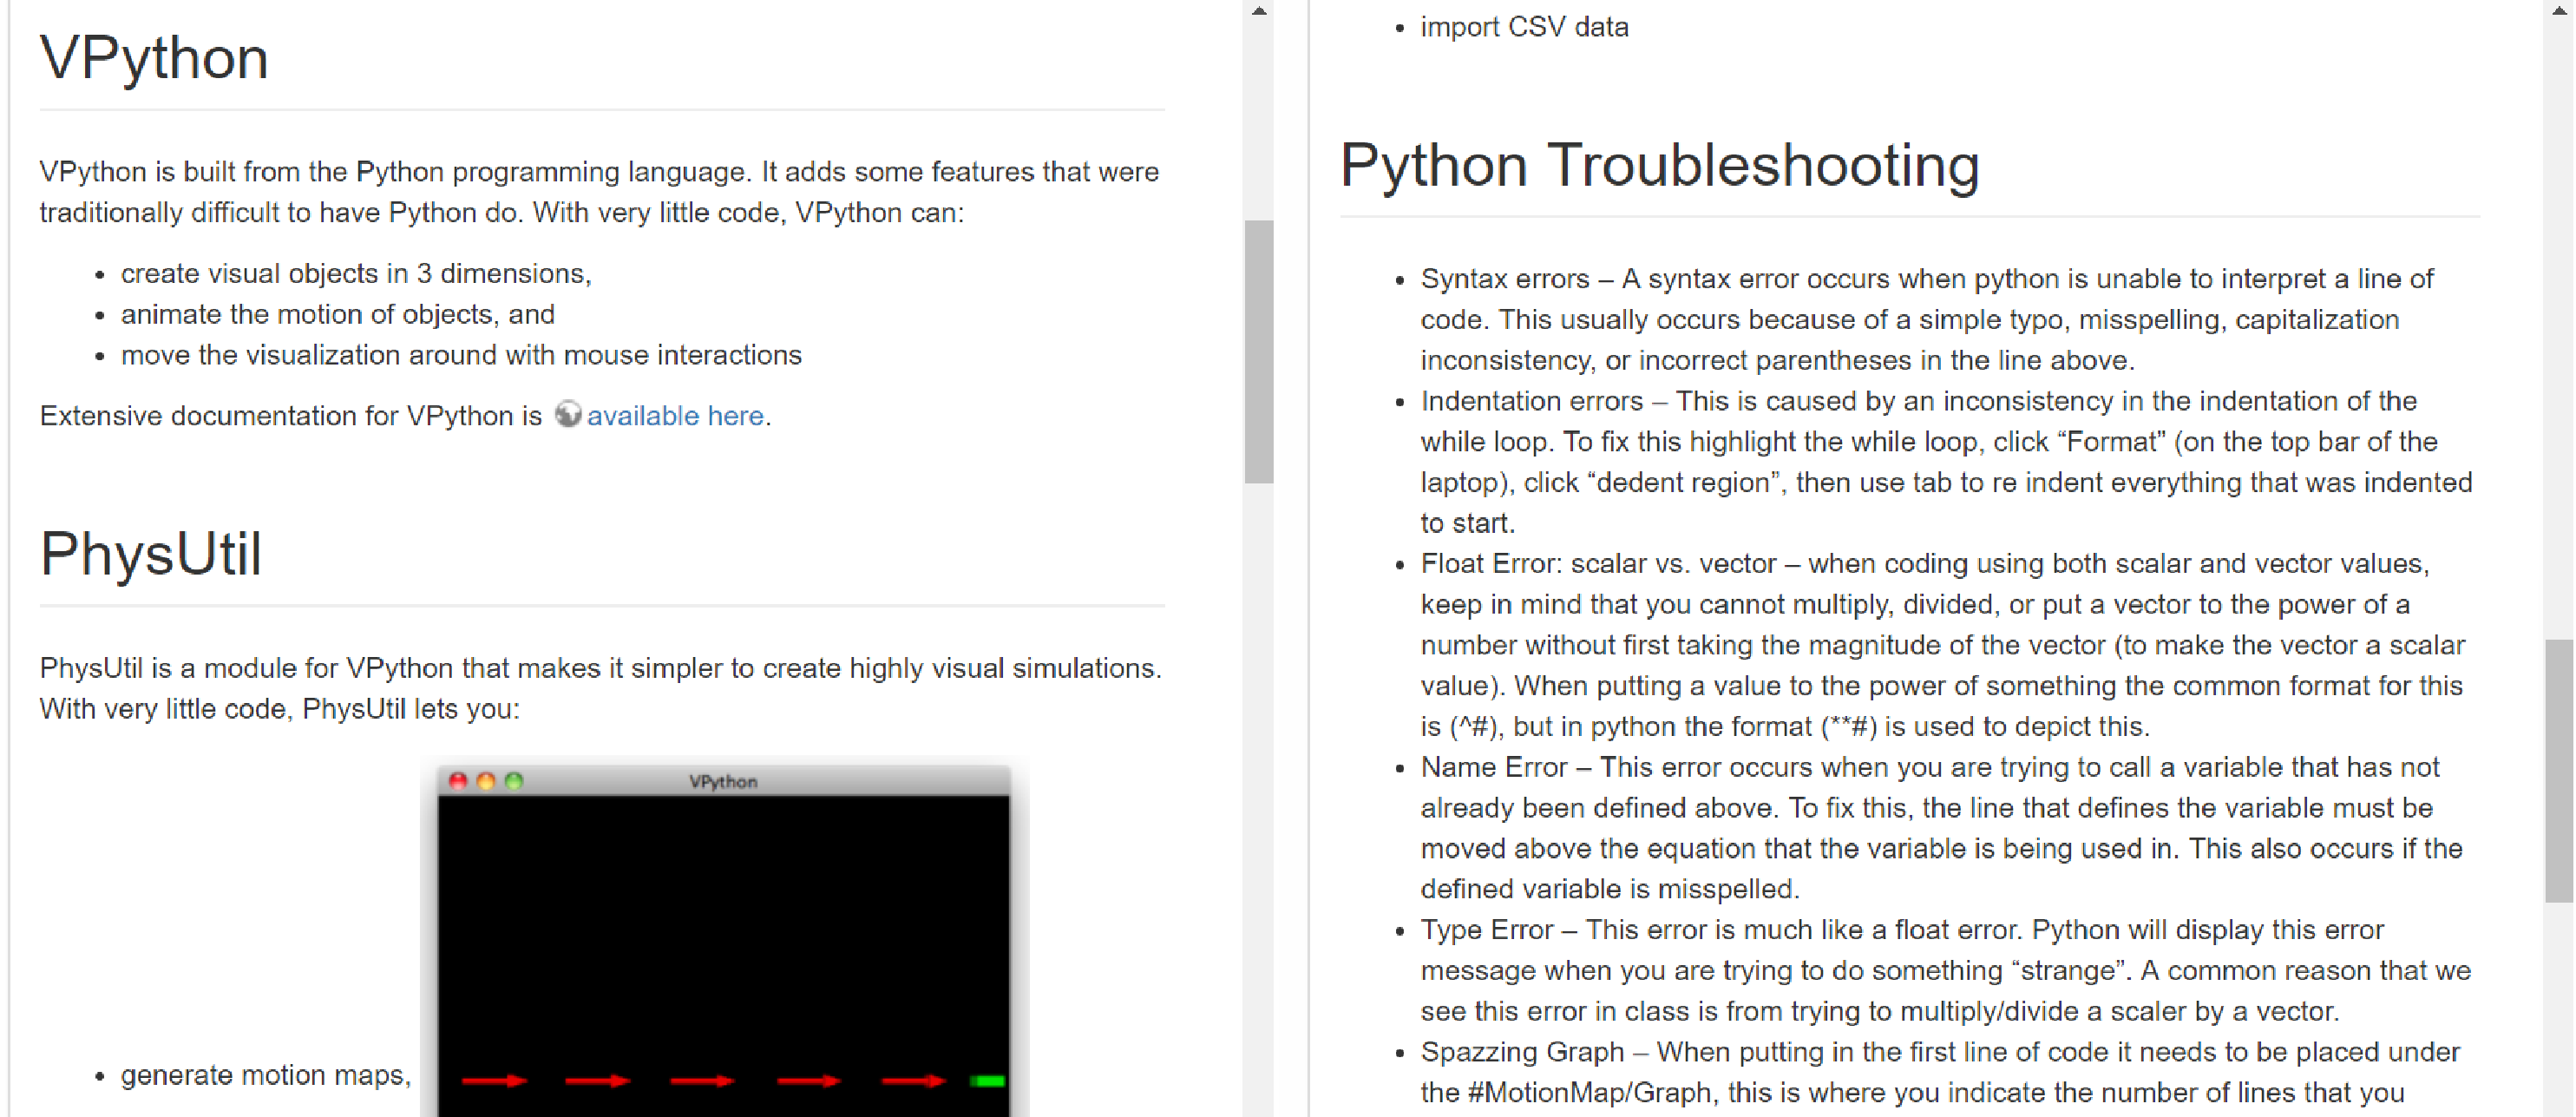
\includegraphics[scale=1]{images/CH3VPythonNotes.pdf}
\caption{Portion of on-line notes that is made available to the students during the first week of the course.  These notes introduce the fundamenatal programming ideas and a list of common errors with tips and tricks.}\label{CH3:VPythonNotes}
\end{figure} 

\section{Pre-class work}

There are other weekly notes, made available to the students at the beginning of every week, focusing more on the fundamental physical ideas that will be used during class.  For example, during the third week the notes focus on uniform circular motion (most heavily used during the week's analytical problem) and the Newtonian gravitational force (most heavily used during the week's computational problem).

Aside from notes, material is also delivered to the students through weekly pre-class homework questions.  Consider the pre-class homework questions shown in Fig.~\ref{CH3:PreClassQuestion} that are made available at the beginning of the third week of the course.  This question is meant to demonstrate that there are multiple correct ways that a unit vector can be constructed in code.  Given the nature of the corresponding week's computational problem (see Sec.~\ref{CH3:SatelliteProblem}), we expect students to be able to draw on and take advantage of this knowledge when faced with a related albeit more complicated problem.  That is, we expect students to be choosing between competing solutions.  Choosing between competing solutions is a problem solving practice indicative of computational thinking that we focused our analysis on.

\begin{figure}[ht]\centering
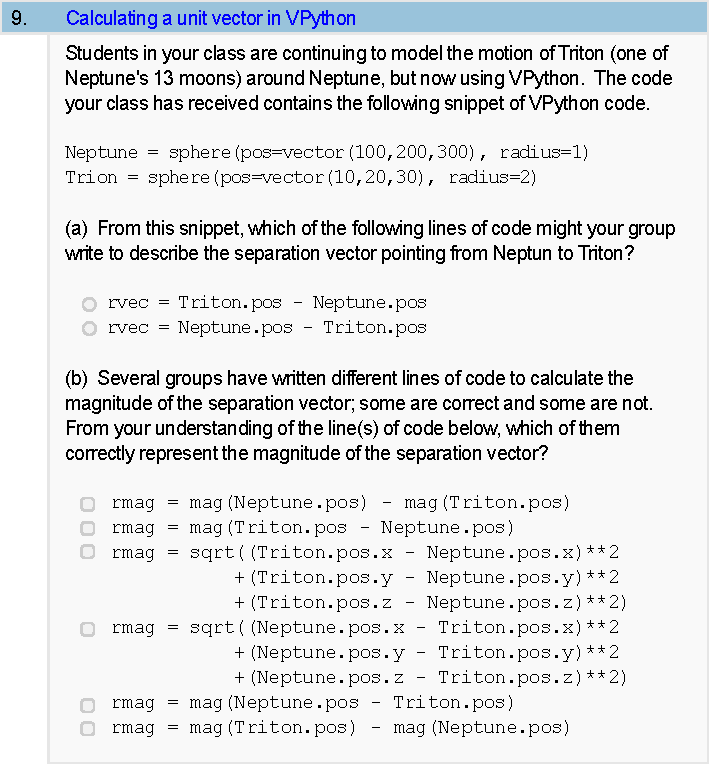
\includegraphics[scale=0.75]{images/CH3PreClassQuestion.pdf}
\caption{Pre-class homework question focusing on the different ways that the magnitude of a vector can be constructed in VPython code: explicitly coding the square root of the sum of the squares of the components and using the pre-defined Python ``magnitude'' function.}\label{CH3:PreClassQuestion}
\end{figure} 

Targeted pre-class homework questions were also developed to help students overcome challenges based on the task analysis.  For example, the pre-class homework questions shown in Fig.~\ref{CH3:PreClassQuestion} were developed to facilitate student understanding of the unit vector of a separation vector between two objects prior to working on the related computational problem.  Given that students must grapple with using a separation vector to construct a unit vector in code during the week, these questions help to place them in the Zone of Proximal Development (ZPD) \cite{Vygotsky1980}.  Constructing computational models is (unsurprisingly) a computational modeling practice indicative of computational thinking that permeates our data.

\section{In-class work}

There are a number of in-class computational problems spread out throughout the semester (see Fig.~\ref{CH3:Schedule}).  The first few computational problems focus on different force models (i.e., no force, a constant force, a non-constant force) and the resulting linear motion of objects.  The last few computational problems focus on extended objects and their rotation.  While solving these problems, groups are expected to engage in a number of computational practices that the problems have been designed around: \begin{enumerate}
\item[P1.] developing and using models,
\item[P2.] planning and carrying out investigations,
\item[P3.] analyzing and interpreting data,
\item[P4.] using mathematics and computational thinking,
\item[P6.] constructing explanations,
\item[P7.] engaging in argument from evidence.
\item[P8.] and obtaining, evaluating, and communicating information.
\end{enumerate}

%\begin{landscape}
%\thispagestyle{empty}
\begin{figure}[ht]\centering

\includegraphics[scale=0.60]{images/CH3Schedule.pdf}
\caption{A schedule for the semester focusing on topics covered, homework/reading deadlines, and in-class problems.  \textbf{Should this figure be on a landscape page?}}\label{CH3:Schedule}
\end{figure}
%\end{landscape}

One of the scientific practices used heavily on both analytic and computation days is that of (P1) developing and using models.  Whether those models be mathematical or computational, we expect students to not only work together in groups to develop the model, but also to utilize that model in further investigations.  This type of scientific practice (P1) and its associated learning goals \cite{Irving2017} were further used to generate the in-class project that this thesis focuses on.

\subsection{Analytic problem}

In the third week of the course, students are asked to analyze the motion of a satellite orbiting Earth both analytically and computationally.  For the analytic day, the groups were asked to solve for the magnitude of the velocity and radius needed by a satellite to be held in a geostationary orbit.  This involves identifying two relevant equations in two unknowns and combining them to solve for the desired radius and magnitude of velocity.  The information gathered during this problem can be used in the following computational problem, and the group facilitators are often observed referencing this information.

\subsection{Computational problem}

This thesis focuses on the third and most complicated computational problem delivered to the students, shown in both Figs.~\ref{CH3:Schedule} and \ref{CH3:SatelliteProblem}. Given its complexity, we developed a framework to help guide and ground our analysis.  This framework was constructed with the help of a task analysis (see Sec.~\ref{CH2:Background}) of the problem.  Ultimately, students must design, construct, and asses a computational model for the Newtonian gravitational force acting on a satellite in geostationary and other more general orbits.

\begin{figure}[ht]\centering
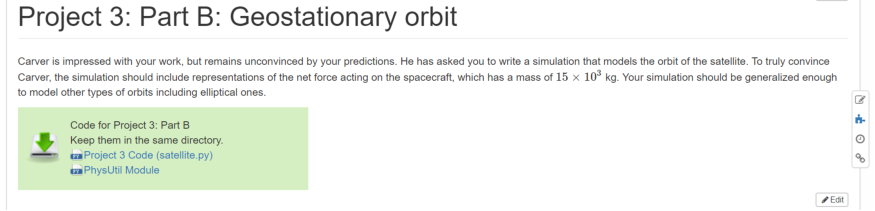
\includegraphics[scale=1]{images/CH3SatelliteProblem.pdf}
\caption{The Newtonian gravitational force problem statement delivered to the students in the third week of class.}\label{CH3:SatelliteProblem}
\end{figure}

Once the correct force has been correctly coded, the group must also grapple with adding in a visualization of a vector representing the force that they have just added.  This type of motion diagram is meant to show that the gravitational force vector resulting in the orbit always points radially inward (toward the Earth).  This task requires students to program as well as allows them to more easily check their conceptual understanding.  Using computational models to understand a concept is a computational modeling and simulation practice that is indicative of computation thinking.

Additionally, in order to check that their model can produce a geostationary orbit, groups are asked to generate a graph showing the magnitude of the separation between the satellite and the center of the Earth vs. time.  This allows them to check for a constant distance which implied a circular orbit.  This task is meant, among other things, to encourage students to visualize data, another computational practice indicative of computational thinking.

\subsubsection{Minimally working programs}

While beginning the problem, the group will observe a Minimally Working Program (MWP) similar to those seen in the two previous computational problems.  This MWP has all of the structure of the code correct (the while/calculation loop and the Euler-Cromer integration) but is missing the computational force acting on the satellite (along with some inaccurate numerical values).  The initial MWP code with its initial visualization are shown in Fig.~\ref{CH3:InitialCodeVisual}.

\begin{figure}[ht]\centering
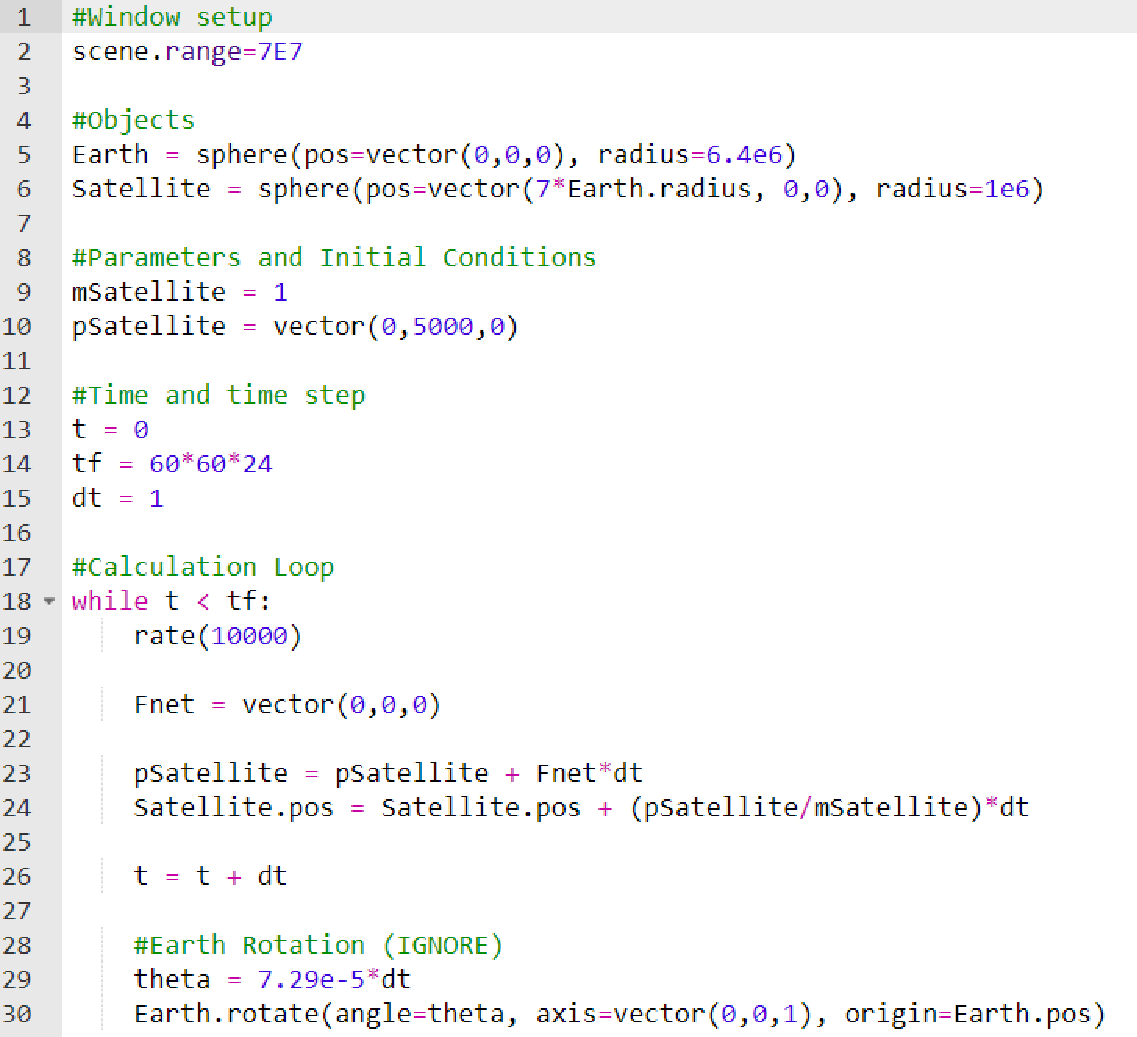
\includegraphics[scale=0.40]{images/CH3InitialCode.pdf}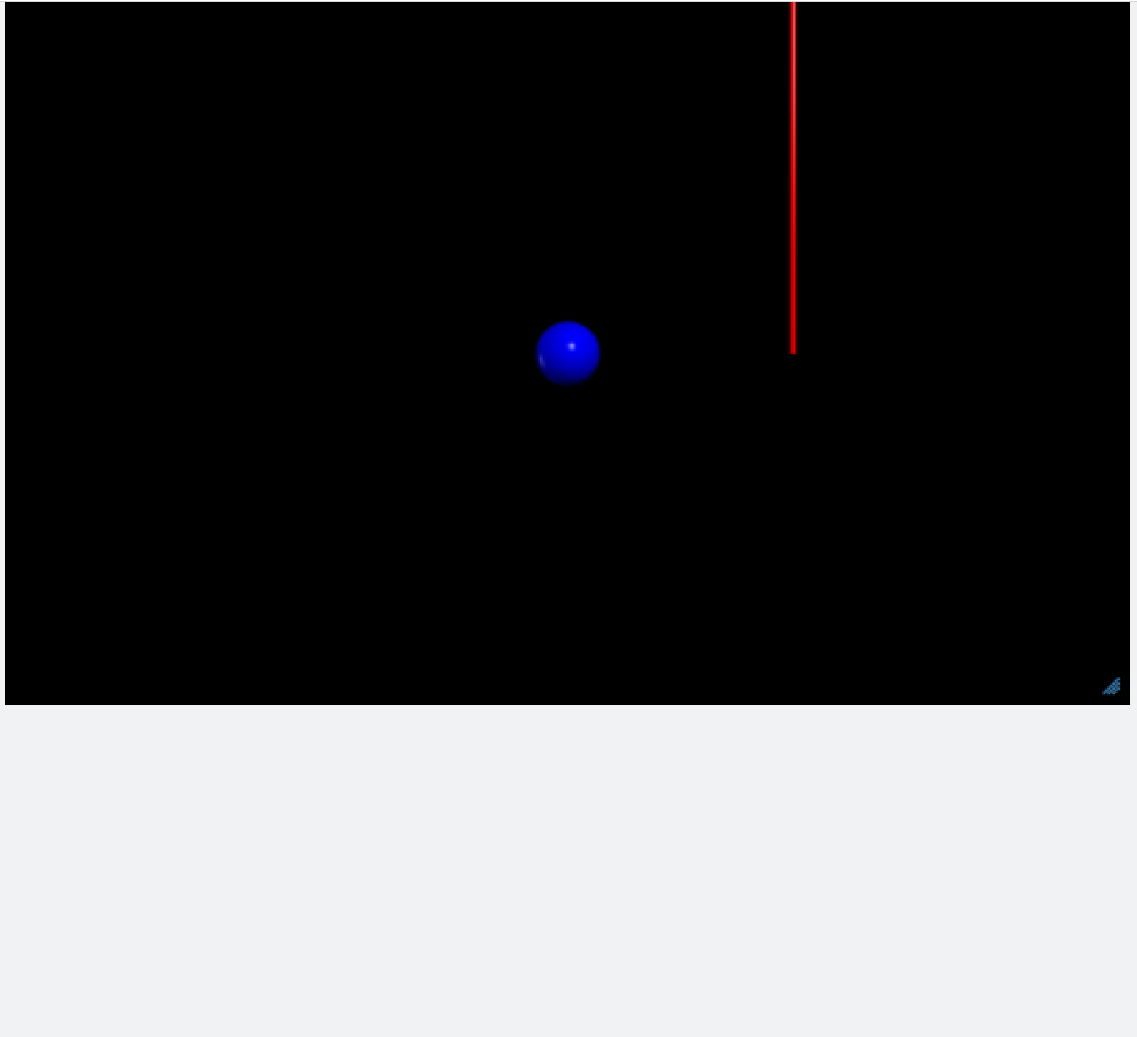
\includegraphics[scale=0.40]{images/CH3InitialVisual.pdf}
\caption{The initial code and visualization of the MWP that is given to the students in the third week of the course.}\label{CH3:InitialCodeVisual}
\end{figure}

Thus, the main task of the group is to construct a physically correct force model in code.  Secondarily, they must modify numerical values to reflect the phenomenon being modeled.  Ideally, this force model will be of a Newtonian gravitational form (i.e., $F_{G}\sim1/r^{2}$) with a direction coded in terms of a separation vector (i.e., $\hat{F}_{G}\sim\vec{r}/r$).  However, there are many other ways to go about this, and we do frequently observe groups working with other models (e.g., a centripetal force).

\subsubsection{Tutor questions}

There are a number of pre-written tutor questions as well as many on-the-fly questions generated by the tutors while in class.  These questions are meant to check the students for conceptual understanding as well as to direct students toward the correct solution.  For example, the tutor questions shown in Fig.~\ref{CH3:TutorQuestion} are meant to ensure that the model the group has constructed is actually general enough to generate all types of elliptical orbits given various initial conditions.

\begin{figure}[ht]\centering
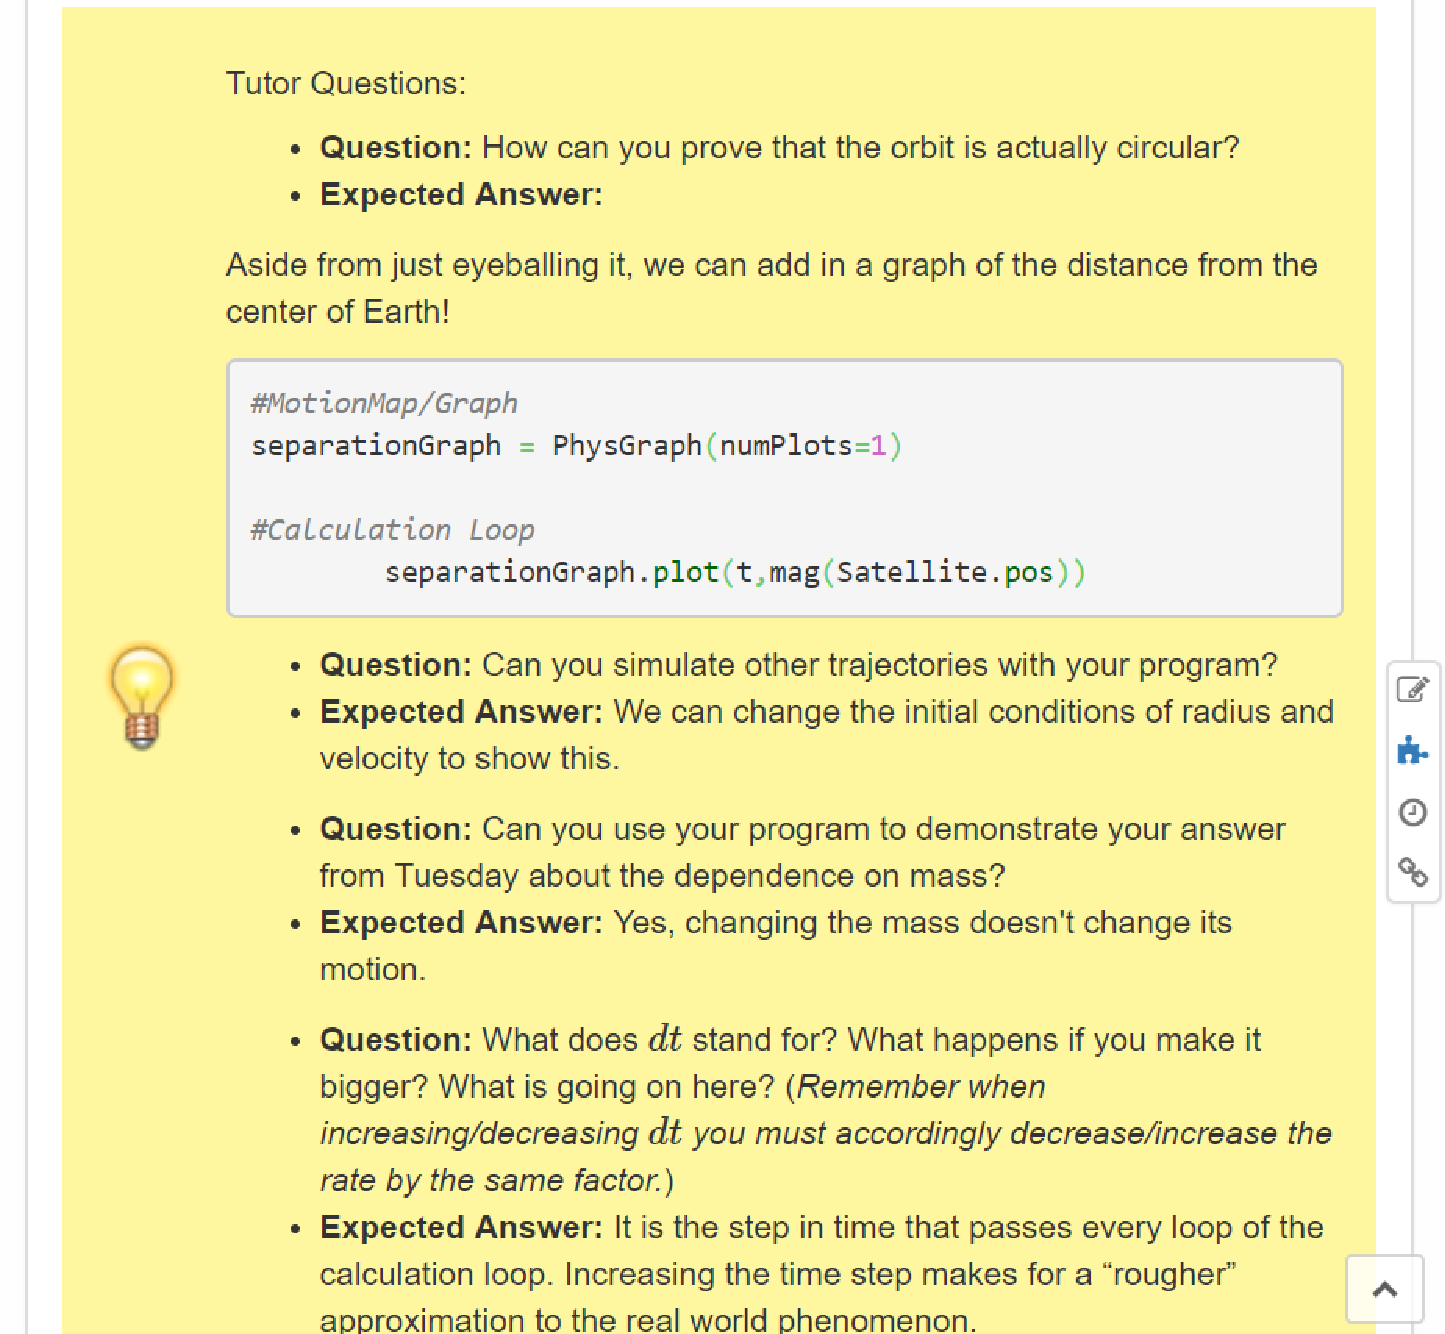
\includegraphics[scale=0.5]{images/CH3TutorQuestion.pdf}
\caption{A seclection of tutor questions that focus on the computational model each group has constructed.}\label{CH3:TutorQuestion}
\end{figure}

On the other hand, a tutor interaction like the one shown below that happens on-the-fly might encourage students to use a more general force rather than a more restricted one:  \begin{description}\TA  you guys wanna talk about what your trategy is at hte moment
\SB  i dont think we know	
\SA we just, we need to figure out how to get the velocity of the spacecraft correct as well as the force net correct and then it should be fine				
\TA yeah, my request, can i point in your program thats what you have for F net now [constant components] my request is to use a completely different strategy where that formula [points to Gmm/r2 on the board] is in for Fnet
\SC yeah we tried to make that yeah		
\SA can we just put the number in?				
\TA umm in principle you could, but id really rather you not have you do it i would like the program to be able to respond if the satellite is father away the force would be less, if the satellite is closer the force would be more so i would like it to be a dynamic program and not one that always have a fixed force\end{description}  In this on-the-fly interaction, the question of weather or not their computational model will be able to handle all types of orbits is enough to indicate that the group needs to switch their model up.  In this way, the tutor is able to make sure the groups stay on the desired path without directly telling them exactly what to do.

\subsection{Feedback/Assessment}

The groups are assessed on many levels in ${\rm P}^{3}$.  One of the most important forms of assessment is given weekly, in the form of written feedback and a numerical score.  The written feedback is based on the observed in-class performance and is designed to point out deficiencies and suggests ways to improve.  The numerical scoring is based on performance in three categories: group understanding, group focus, and individual understanding.

Often the written feedback pertains to group activity with the computer.  For example, the portion of written feedback shown in Fig.~\ref{CH3:WrittenFeedback} is encouraging a student to allow other group members to do some of the typing.   This could be requested for any number of reasons -- most likely, though, because the students with less prior programming experience are not being given a chance to participate.

\begin{figure}[ht]\centering
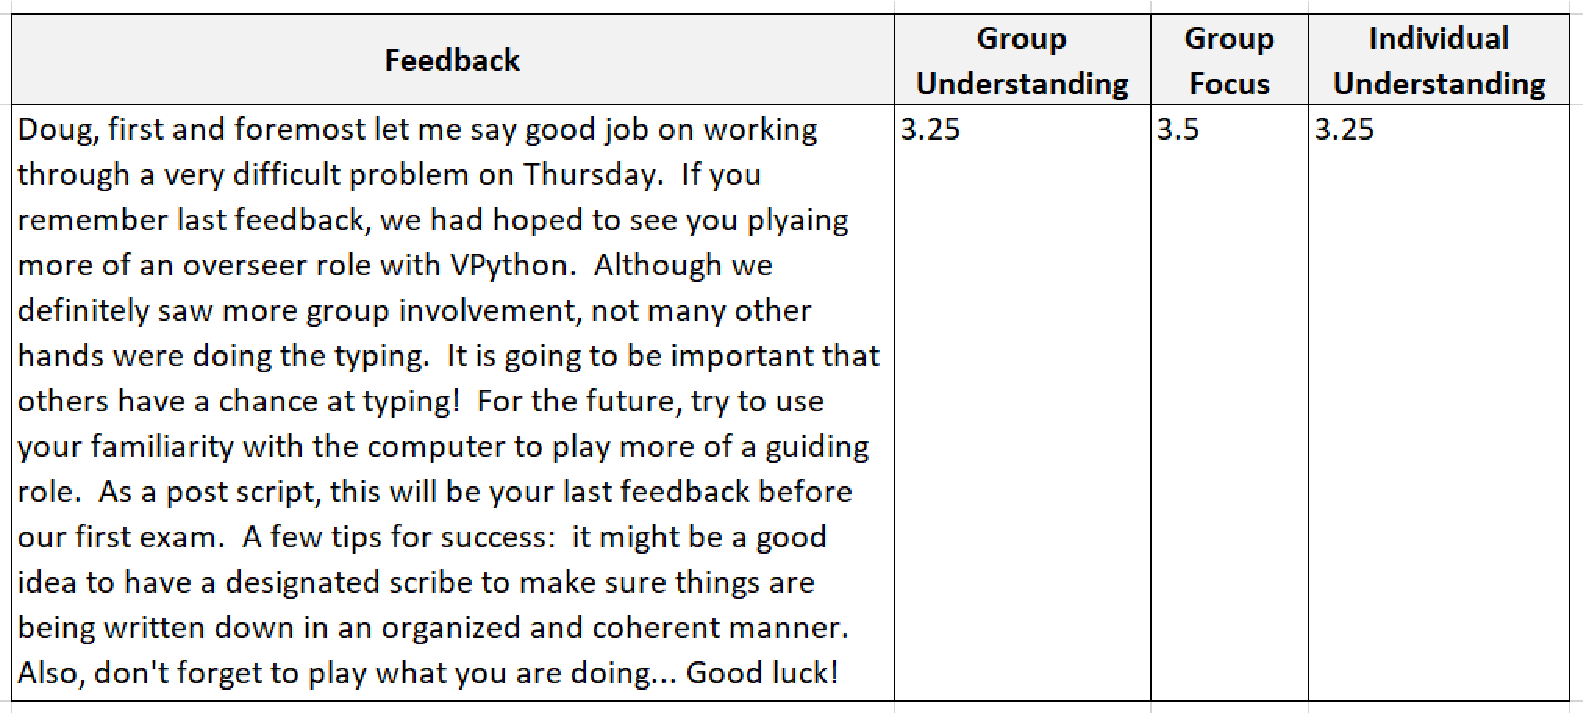
\includegraphics[scale=1.25]{images/CH3WrittenFeedback.pdf}
\caption{A snippet of written feedback given to a student after the third week.}\label{CH3:WrittenFeedback}
\end{figure}

In this way, instructors can encourage their groups to share the programming load.  While doing the typing, it is very difficult to follow along without knowing exactly what is going on.  This helps to engage all of the students with the material.

\section{Post-class work}

There are a number of post-class homework questions that are meant to reinforce the physics and computational concepts seen in class.  During the third week of the course, these questions focus mostly on the Newtonian gravitational force.  However, the post-class homework question shown in Fig.~\ref{CH3:PostClassHomework} that is delivered in the third week focuses on the previous week's computational problem (i.e., it involves a local gravitational force as opposed to a Newtonian gravitational force).  Nevertheless, this post-class question involves the same Euler-Cromer style of numerical integration as seen in all computational problems.  The students are expected to use the error message in order to identify an error in the code.

\begin{figure}[ht]\centering
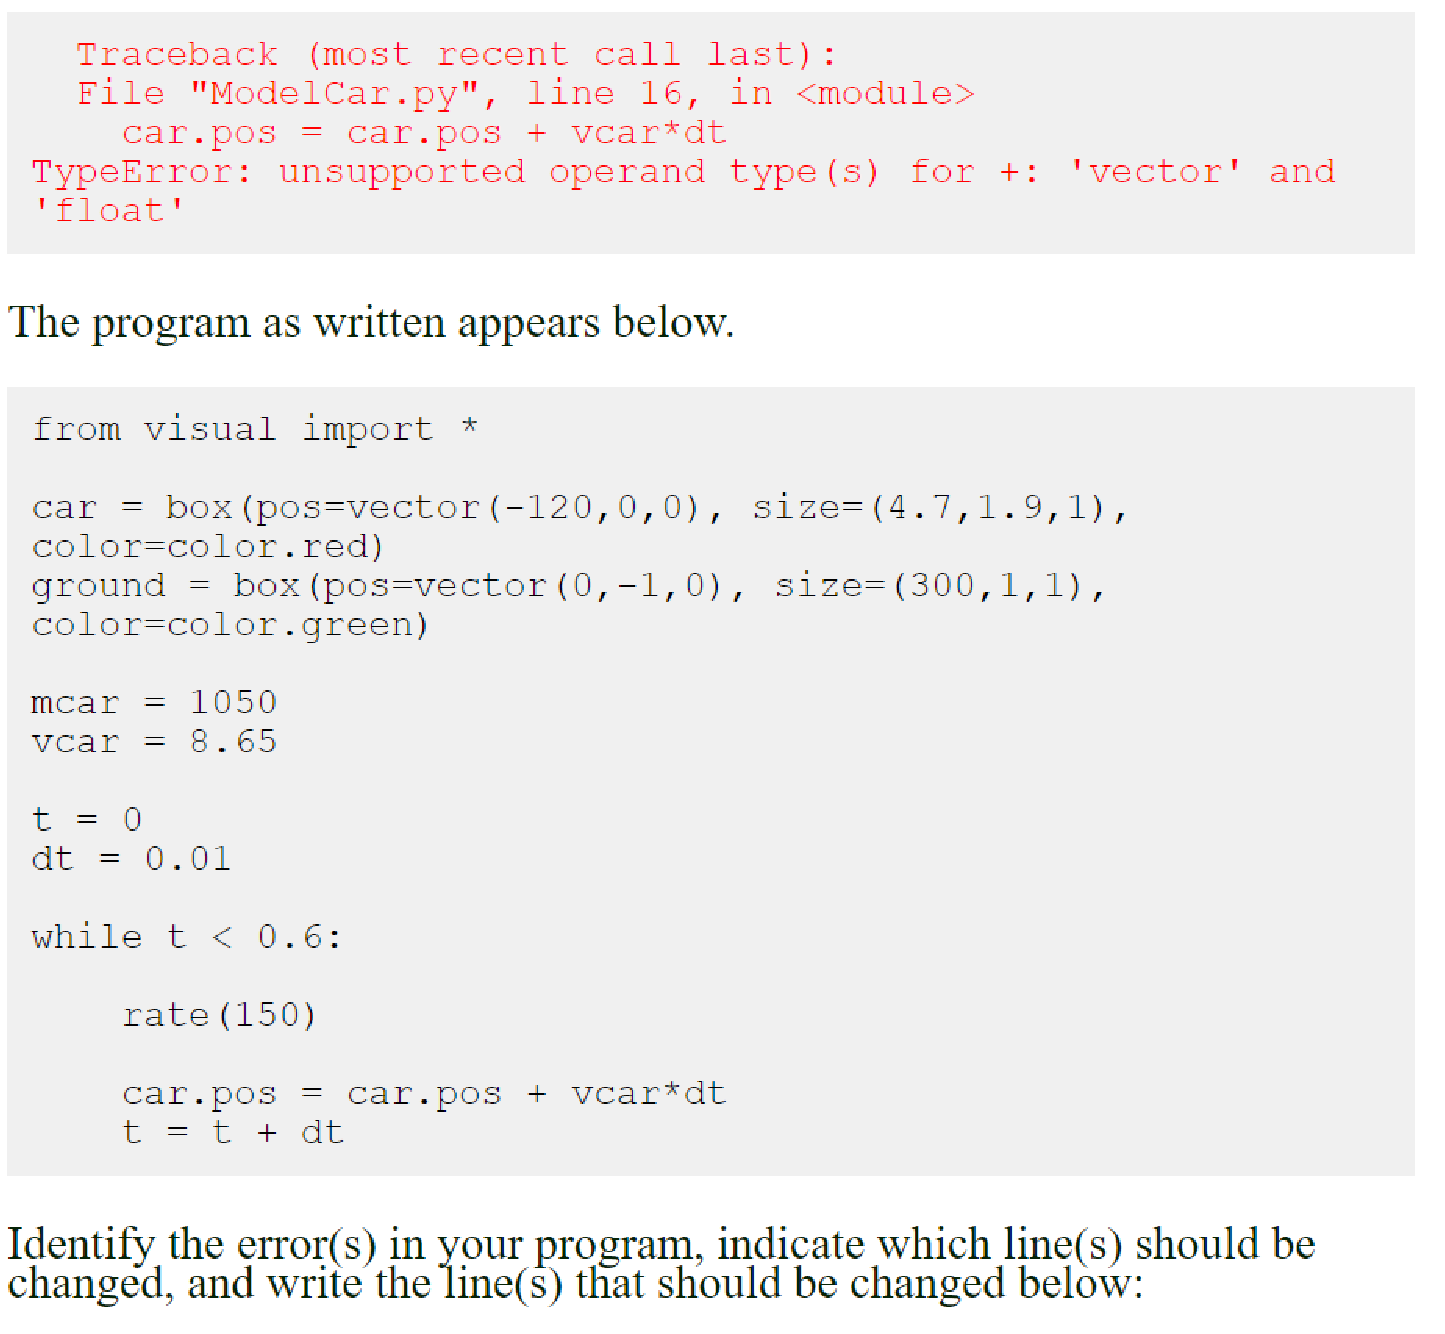
\includegraphics[scale=0.50]{images/CH3PostClassHomework.pdf}
\caption{A portion of a post-class homework question delivered in the third week of the course.  This question requires students to troubleshoot and debug the code.}\label{CH3:PostClassHomework}
\end{figure}

This type of problem helps to encourage students to identify, isolate, reproduce, and correct unexpected problems that arise while constructing computational models.  Ideally, it requires students to interpret the names given to the variables being used and verify that they are defined in a correct form.  Correct form means following one of the basic rules of algebra -- you cannot add a scalar and a vector.

%
%	MOTIVATION
%

\chapter{Motivation}\label{CH4:Motivation}

Aside from a general interest in introductory computational physics, it is important to understand the underlying motivation(s) for this thesis.

The process of identifying an interesting computational practice, described in Sec.~\ref{Sec:Debug}, was the earliest motivation for this study.  We found that it was extremely difficult to define and identify the particular practice of what we named ``physics debugging.''  Not only did the practice need to be clearly defined, it also needed to be clearly identified in the data.  This required a lot of in-depth qualitative analysis and inter-rater reliability, motivating our use of the Weintrop framework and the qualitative methods of Clarke et. al.

Additionally, as described in Sec.~\ref{Sec:Phenom}, we found that it was very difficult to understand the qualitatively different ways in which students experienced computational introductory physics.  This difficulty motivated a task analysis with a focus on identifying practices that the students were engaging in through in-class observation, as opposed to their experiences through out-of-class interviews.
  
\section{Debugging}\label{Sec:Debug}

In this section, we present a case study of a group of students immersed in this ${\rm P}^{3}$ environment solving a computational problem.  This problem requires the translation of a number of fundamental physics principles into computer code.  Our analysis consists of qualitative observations in an attempt to describe, rather than generalize, the computational interactions, debugging strategies, and learning opportunities unique to this novel environment.

We focus this case study on the interactions between group and computer to begin to understand the ways in which computation can influence learning.  Particularly, we are interested in the interactions occurring simultaneously with social exchanges of fundamental physics principles (FPPs) specific to the present task (e.g., discussing $d\mathbf{r}=\mathbf{v}\,dt$ on a motion task) and the display of desirable problem solving strategies (e.g., divide-and-conquer).  These group-computer interactions vary in form, from the more active process of sifting through lines of code, to the more passive process of observing a three-dimensional visual display.

One previously defined computational interaction that reinforces desirable strategies, borrowing from computer science education research, is the process of debugging \cite{Fitzgerald2008}.  Computer science defines debugging as a process that comes after testing \emph{syntactically} correct code where programmers ``find out exactly where the error is and how to fix it. \cite{McCauley2008}''  Given the generic nature of the application of computation in computer science environments (e.g., data sorting, poker statistics, or ``Hello, World!'' tasks), we expect to see unique strategies specific to a computational \emph{physics} environment.  Thus, we extend this notion of computer science debugging into a physics context to help uncover the strategies employed while groups of students debug \emph{fundamentally} correct code that produces unexpected physical results.

\subsection{Analysis}

In Fall 2014, ${\rm P}^{3}$ was run at Michigan State University in the Physics Department.  It was this first semester where we collected \emph{in situ} data using three sets of video camera, microphone, and laptop with screencasting software to document three different groups each week.  From the subset of this data containing computational problems, we \emph{purposefully sampled} a particularly interesting group in terms of their computational interactions, as identified by their instructor.  That is, we chose our case study not based on generalizability, but rather on the group's receptive and engaging nature with the project as an \emph{extreme case}.\cite{Flyvbjerg2006}

The project that the selected group worked on for this study consists of creating a computational model to simulate the geosynchronous orbit of a satellite around Earth.  In order to generate a simulation that produced the desired output, the group had to incorporate a position dependent Newtonian gravitational force and the update of momentum, using realistic numerical values.  The appropriate numerical values are Googleable, though instructors encouraged groups to solve for them analytically.

This study focuses on one group in the fourth week of class (the fourth computational problem seen) consisting of four individuals: Students A, B, C, and D.  The group had primary interaction with one assigned instructor.  Broadly, we see a 50/50 split on gender, with one ESL international student.  Student A had the most programming experience out of the group.  It is through the audiovisual and screencast documentation of this group's interaction with each other and with the technology available that we began our analysis.

To focus in on the group's successful physics debugging occurring over the $\SI{2}{\hour}$ class period, we needed to identify phases in time when the group had recognized and resolved a physics bug.  These two phases in time, \emph{bug recognition} and \emph{bug resolution} are the necessary limits on either side of the process of \emph{physics debugging}, as represented in Fig.~\ref{CH4:Phases}.  We identified these two bounding phases at around $\SI{60(5)}{\minute}$ into the problem, and further examined the process of debugging in-between.  That is, we focused on the crucial moments surrounding the final modifications that took the code from producing unexpected output to expected output.

\begin{figure}\centering
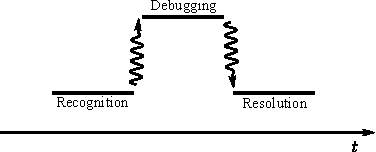
\includegraphics[scale=1]{./images/phases.pdf}
\caption{The debugging process necessarily corresponds to a phase beset on either side by the phases of recognition and resolution.  Note the absence of a vertical scale, as the vertical separation merely acts to distinguish phases.}\label{CH4:Phases}
\end{figure}

\subsubsection{Recognition}

\subsubsection{Resolution}

\section{Phenomenography}\label{Sec:Phenom}

A description of the phenomenography study.

\subsection{Protocol}

A description of the development of the protocol.

\subsection{Analysis}

Since there are no real results, we can just describe how we analyzed the interview data.

%
%	ANALYSIS
%

\chapter{Analysis}\label{CH5:Analysis}

\section{Specific methods}

Following the suggestion of thematic analysis, we begin with a full transcription of the in-class video.  This transcription is verbatim to the best of our abilities.  Any inaudible sections are indicated, with long pauses being indicated by ellipses ($\ldots$).  To distingish between unspoken actions (e.g., pointing to an equation) and infereces made by the researcher (e.g., refering to a previous equation), we follow the convention of square brackets ($[\,]$) and curly brackets ($\{\,\}$), respectively.

This full transcript is then read through multiple times, noting any points of interest in terms of the Weintrop framework.  We then divide the transcript into multiple excerpts of shorter length centered around the initial points of interest.  Although we lose some of the coherence of the problem as a whole by focusing on shorter exerpts, these relatively shorter exerpts help to facilitate a deeper analysis.  Each transcript contains $\approx\SI{1500}{lines}$ comprising $\approx\SI{50}{excerpts}$.

Each excerpt is analyzed in terms of the practices the group is engaging in.  This means we need to look for the characteristics of each practice. With these characteristics identified, we are justified in classifying the particular excerpt as that practice.  Each excerpt generally has between one and four identified computational practices. 

Each characteristic that is identified is supported with rationale on three levels: the rationale according to the framework, the rationale within the excerpt, and the rationale beyond the excerpt.  The confidence in this rationale (specifically, the rationale within the excerpt) manifests itself in a high, medium, and low confidence rating for the identification of this practice.  In that way, we know not only how frequently the practices are identified, but also how confident we are in that assessment.

\begin{figure}[ht]\centering
%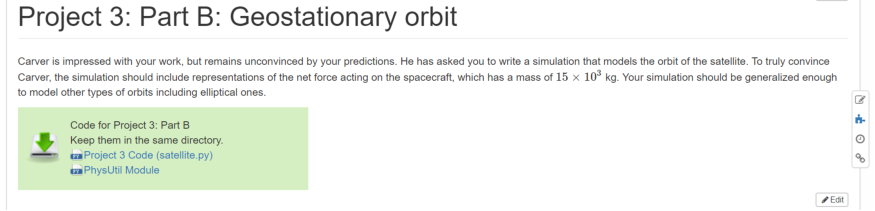
\includegraphics[scale=1]{images/CH3SatelliteProblem.pdf}
\caption{Visual representation of the different levels of rationale pertaining to an excerpt.  Green, yellow, and red cells represent high, medium, and low confidence, respectively.}\label{CH3:VariableAnalysis}
\end{figure}

So that we safeguard against the researcher influencing the results too much, inter-rater reliability is checked at multiple points throughout the analysis.  This check consists of an independent researcher (the inter-rater) identifying practices with confidence in a reduced set of the data and comparing with the primary researcher.  Any practices in which confidence is questioned and lost are discounted from being identified.

\section{Findings}

Recall that, according to the framework, each category of practice can be broken down into a number of individual practices.  Each individual practice, further, can be identified in terms of a number of fundamental characteristics.  Depending on the particular situation, some categories show up in the data more often than others.  For example, we expect to see fewer systems thinking practices and more computational modeling practices.  Further, within any category, some individual practices show up in the data more than others.  For example, within the data practices, we expect to see fewer instances of collecting data and more instances of creating data.

Most importantly, within any individual practice, there is a broad set of defining characteristics.  Ideally, each characteristic would be present in some form when its corresponding practice has been identified.  However, each characteristic can be organized in terms of being either necessary or sufficient for the cause.  That is, we need not necessarily observe every characteristic in order to identify a practice according to the framework.

\begin{figure}[ht]\centering
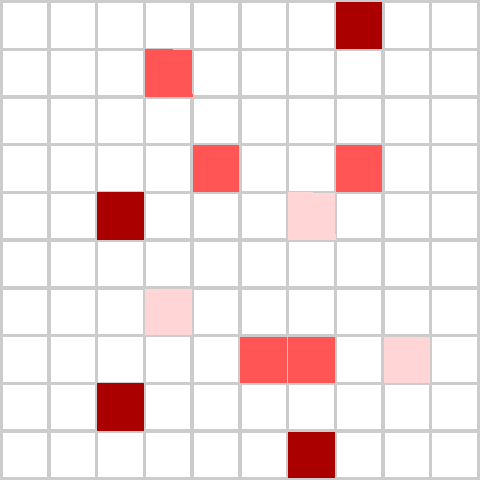
\includegraphics[scale=1]{./images/matrix.pdf}
\caption{A ``density plot'' for all computational practices and all groups.}\label{CH5:DensityPlot}
\end{figure}

\subsection{Assessing computational models}

The most important computational modeling practice indicative of computational thinking is that of assessing computational models.  This practice shows up $\SI{100}{\percent}$ of the time.  Assessing computational models seems to be crucial to the process of designing and constructing computational models.  Given that computational models take a lot of work and iteration to get to an acceptable level, it is no surprise that assessing shows up so frequently.

There are three characteristics that are necessary to be observed in an excerpt to warrant classification of ``assessing computational models.''  The first characteristic that needs to be observed is a ``model.''  There are several models that show up in the data.  The second characteristic that needs to be observed is a ``phenomenon.''  For the most part, the phenomena are related to the simulation of the trajectory of the geostationary satellite and its various physical interpretations (e.g., a central attractive force or a circular orbit).  The third characteristic that needs to be observed is a ``comparion'' between the model and phenomenon.  The comparisons that we see are ultimately varied, given that they depend on not only the model but also the phenomenon.

\begin{figure}[ht]\centering
\begin{tabular}{l|c|r}
a & b & c \\\hline
c & d & $\SI{100}{\percent}$ \\
\end{tabular}
\caption{A table showing rough statistics for assessing computational models.}\label{CH5:AssessingComputationalModels}
\end{figure}

\subsubsection{Computational model}

The two big models that we have observed in the data are a position dependent Newtonian gravitational force in terms of a separation vector and a centripetal force that depends on the polar angle of the satellite.  Each model shows up $\SI{100}{\percent}$ and $\SI{100}{\percent}$ of the time, respectively.

\subsubsection{Phenomenon}

The phenomena that we have observed in the data are almost always centered around the simulation of the trajectory of the satellite.  The physical interpretations of the phenomena are, not surprisingly, closely related to the topics covered in the couse notes and the topics questioned in the weekly homework.  These interpretations range from the crude (e.g., a circular orbit) to the sophisticated (e.g. a centripetal force and its properties).  This variety of phenomena show up $\SI{100}{\percent}$ of the time.

\subsubsection{Comparison between}

The comparisons that we have observed in the data are quite varied.  Given that the comparison is between the models and phenomena, we expect this characteristic to be the most varied.

\subsection{Creating data}

\subsubsection{Data set}

\subsubsection{Algorithmic procedure}

\subsubsection{Advance understanding}

%
%	DISCUSSION
%

\chapter{Discussion}\label{CH6:Discussion}


\section{Primary practices}

Analyzing data, assessing computational models, programming, and thinking in levels are the most common practices that we observed.

\section{Secondary practices}

Creating data, constructing computational models, creating computational abstractions, and understanding the realations within a system are the lesser common practices that we observed.

\section{Absent practices}

Some of the practices that were not observed in the data were collecting data and choosing effective computational tools.

%
%	CONCLUSIONS
%

\chapter{Conclusion}\label{CH7:Conclusion}

The most important things that you should be paying attention to are the creation and analysis of data, the assessment and construction of models, programming and troubleshooting, and thinking in levels and communicating

%
%	APPENDICES
%

\appendices

\chapter{Additional excerpts}

%
%	BIBLIOGRAPHY
%

\end{doublespace}

\bibliography{bibliography}
\bibliographystyle{plain}

\end{document}

%
%	EXTRA
%

%\begin{landscape}
%\thispagestyle{empty}
%\captionof{table}{caption_text}
%\captionof{figure}{caption_text}
%\end{landscape}